%% Template para dissertação/tese na classe UFPEthesis
%% versão 0.9.2
%% (c) 2005 Paulo G. S. Fonseca
%% www.cin.ufpe.br/~paguso/ufpethesis

%% Carrega a classe ufpethesis
%% Opções: * Idiomas
%%           pt   - português (padrão)
%%           en   - inglês
%%         * Tipo do Texto
%%           bsc  - para monografias de graduação
%%           msc  - para dissertações de mestrado (padrão)
%%           qual - exame de qualificação doutorado
%%           prop - proposta de tese doutorado
%%           phd  - para teses de doutorado
%%         * Mídia
%%           scr  - para versão eletrônica (PDF) / consulte o guia do usuario
%%         * Estilo
%%           classic - estilo original à la TAOCP (deprecated)
%%           std     - novo estilo à la CUP (padrão)
%%         * Paginação
%%           oneside - para impressão em face única
%%           twoside - para impressão em frente e verso (padrão)

%% Preâmbulo:
%% coloque aqui o seu preâmbulo LaTeX, i.e., declaração de pacotes,
%% (re)definições de macros, medidas, etc.
\documentclass[bsc, oneside]{UFPEThesis/ufpethesis}
\usepackage[table]{xcolor}
\usepackage{multirow}
\usepackage{makecell}
\usepackage{caption}
\usepackage{subcaption}
\usepackage{hyperref}

%% Identificação:

% Universidade
% e.g. \university{Universidade de Campinas}
% Na UFPE, comente a linha a seguir
\university{Universidade Federal de Pernambuco}

% Endereço (cidade)
% e.g. \address{Campinas}
% Na UFPE, comente a linha a seguir
% \address{<CIDADE DA IES>}

% Instituto ou Centro Acadêmico
% e.g. \institute{Centro de Ciências Exatas e da Natureza}
% Comente se não se aplicar
\institute{Centro de Informática}

% Departamento acadêmico
% e.g. \department{Departamento de Informática}
% Comente se não se aplicar
% \department{<NOME DO DEPARTAMENTO>}

% Programa de pós-graduação
% e.g. \program{Pós-graduação em Ciência da Computação}
\program{Bacharelado em Ciência da Computação}

% Área de titulação
% e.g. \majorfield{Ciência da Computação}
\majorfield{Ciência da Computação}

% Título da dissertação/tese
% e.g. \title{Sobre a conjectura $P=NP$}
\title{Uma adaptação do \textit{Client-Side Prediction} para ambientes musicais colaborativos \textit{online}}

% Data da defesa
% e.g. \date{19 de fevereiro de 2003}
% \date{<DATA DA DEFESA>}

% Autor
% e.g. \author{José da Silva}
\author{Luiz Henrique Tavares Caúla}

% Orientador(a)
% Opção: [f] - para orientador do sexo feminino
% e.g. \adviser[f]{Profa. Dra. Maria Santos}
\adviser{Filipe Carlos de Albuquerque Calegario}

% Orientador(a)
% Opção: [f] - para orientador do sexo feminino
% e.g. \coadviser{Prof. Dr. Pedro Pedreira}
% Comente se não se aplicar
% \coadviser{NOME DO(DA) CO-ORIENTADOR(A)}

%% Inicio do documento
\begin{document}

%%
%% Parte pré-textual
%%
\frontmatter

% Folha de rosto
% Comente para ocultar
\frontpage

% Portada (apresentação)
% Comente para ocultar
\presentationpage

% Dedicatória
% Comente para ocultar
% \begin{dedicatory}
% <DIGITE A DEDICATÒRIA AQUI>
% \end{dedicatory}

% Agradecimentos
% Se preferir, crie um arquivo à parte e o inclua via \include{}
\acknowledgements

TODO: Agradecimentos

% Epígrafe
% Comente para ocultar
% e.g.
%  \begin{epigraph}[Tarde, 1919]{Olavo Bilac}
%  Última flor do Lácio, inculta e bela,\\
%  És, a um tempo, esplendor e sepultura;\\
%  Ouro nativo, que, na ganga impura,\\
%  A bruta mina entre os cascalhos vela.
%  \end{epigraph}
% \begin{epigraph}[<NOTA>]{<AUTOR>}
% <DIGITE AQUI A CITAÇÂO>
% \end{epigraph}

% Resumo em Português
% Se preferir, crie um arquivo à parte e o inclua via \include{}
\resumo
\addcontentsline{toc}{chapter}{Resumo}

Devido à alta sensibilidade do aparelho auditivo humano, para performar em conjunto com outros artistas, músicos necessitam que haja pouca latência entre a saída dos instrumentos de seus colegas e seu retorno. Dessa forma, proporcionar um ambiente colaborativo em tempo real via Internet torna-se um desafio pertinente na área de Computação Musical e Rede de Computadores. Algumas soluções procuram otimizar a conexão entre os computadores construindo infraestruturas dedicadas ou abandonam o requisito de tempo real ao entregar experiências assíncronas. No entanto, tais abordagens não abrangem, de forma síncrona, casos em que não haja acesso a uma conexão de alta velocidade ou que exista uma grande distância entre os participantes.

Este trabalho propõe, dessa forma, uma adaptação do algoritmo \textit{Client-Side Prediction}, utilizado em \textit{videogames online}, experimentando dois modelos preditivos para gerar novas sequências de áudio baseando-se nas anteriores - predição de sequências com LSTM (\textit{Long Short-Term Memory}) e indexação e identificação de sequências com DTW (\textit{Dynamic Time Warping}). De tal forma, espera-se que, não sendo necessária a espera pela saída do cliente transmissor, haja uma redução da percepção de latência por parte dos participantes.

Utilizando duas métricas de sucesso - corretude das previsões e tempo de processamento - avaliamos que o modelo gerador com LSTM não performou bem comparado ao modelo indexador com DTW, que apresentou resultados bastante promissores e que pode ser utilizado para músicas de gêneros com tendências menos improvisacionais.

\begin{keywords}
latência, áudio, predição de sequência, streaming, transmissão, online, música, client-side prediction, rollback, dtw, lstm
\end{keywords}


% Resumo em Inglês
% Se preferir, crie um arquivo à parte e o inclua via \include{}
% \abstract
% Palavras-chave do resumo em Inglês
% \begin{keywords}
% <DIGITE AS PALAVRAS-CHAVE AQUI>
% \end{keywords}

% Sumário
% Comente para ocultar
\tableofcontents

% Lista de figuras
% Comente para ocultar
\listoffigures

% Lista de tabelas
% Comente para ocultar
\listoftables



%%
%% Parte textual
%%
\mainmatter

% É aconselhável criar cada capítulo em um arquivo à parte, digamos
% "capitulo1.tex", "capitulo2.tex", ... "capituloN.tex" e depois
% incluí-los com:
\chapter{Introdução}

A performance artística musical, quando praticada em conjunto, requer alto nível de colaboração entre os participantes. Em música, sobretudo gêneros com tendências improvisacionais como \textit{jazz}, \textit{blues} e \textit{rock}, o ato de ouvir e reagir ao som de seus companheiros é tão importante quanto aquele produzido individualmente. Dessa forma, o \textit{feedback} auditivo de baixa latência dos instrumentos tocados é fundamental para que haja uma sensação fluida entre os participantes.

Normalmente, músicos performando em conjunto em um mesmo ambiente físico raramente experienciarão problemas relacionados à latência. No entanto, em um contexto de distanciamento social, encorajado durante à Pandemia de COVID-19 no ano de 2020, músicos ao redor do mundo viram-se obrigados a transferirem esse ambiente para um virtual \textit{online}.

% Devido à abordagem de "melhor esforço" em que a Internet foi originalmente projetada - sob a suposição de que não é possível garantir o recebimento de todos os pacotes transmitidos - protocolos de transmissão de voz como \textit{VoIP} (\textit{Voice over Internet Protocol}) e serviços provedores videoconferências necessitam implementar medidas compensatórias, como grandes \textit{buffers} de rede e retransmissão de pacotes. Tais medidas, consequentemente, garantem a corretude dos dados transmitidos, sob o custo do aumento na latência total \cite{carot_low_latency}. Para aplicações comuns, essa troca é aceitável; entretanto, no contexto da arte musical colaborativa, mostra-se inviável.

Aplicações comerciais de videoconferências, como o \textit{Zoom}, \textit{Google Meet} e \textit{FaceTime}  possuem sensibilidade de tempo para manter conversas compreensíveis - a \textit{Cisco} define a latência máxima aceitável de uma implementação \textit{VoIP} em até 150 ms \cite{cisco}. Este limite, apesar de relativamente baixo, pode ser alcançado por conexões de velocidades medianas, implementações de processamento de áudio e infraestruturas de rede compartilhadas. No entanto, para a prática colaborativa musical, onde tolerância máxima é bastante restrita - variando entre 10 ms e 55 ms \cite{mcphearson} - mostra-se inviável. Em ambientes de alta latência, músicos tendem a perceber incômodos e mudam a forma sobre como performam para adptarem-se. \cite{carot_low_latency}.

Para lidar com estes problemas, \textit{softwares} voltados especificamente para a colaboração musical \textit{online} apresentam uma variedade de abordagens diferentes. \textit{LoLa} \cite{lola}, \textit{SoundJack} \cite{soundjack} e \textit{JamKazam} \cite{jamkazam}, por exemplo, implementam otimizações na camada de rede - como conectar clientes diretamente entre si via \textit{P2P} (\textit{peer-to-peer}) - oferecendo latências aceitáveis entre distâncias medianas. Outras aplicações, como o \textit{Jammr} \cite{jammr}, dispensam o requisito de tempo real e apresentam soluções assíncronas, onde os músicos ouvem os últimos quatro compassos tocados por seus companheiros em um \textit{loop} contínuo.

No entanto, tais abordagens não abrangem casos onde não é possível ter acesso a conexões dedicadas ou os músicos residem entre grandes distâncias, ainda mantendo uma performance síncrona.

Ao observar o contexto de videogames, encontramos requisitos de latência similares. Gêneros que utilizam reações como mecânica de jogabilidade, como luta e FPS (\textit{first-person shooter}), para oferecerem aos jogadores uma experiência fluida, necessitam de latências máximas de até 100 ms \cite{pubnub}. O algoritmo mais popular e efetivo para solucionar esse problema, \textit{Rollback Netcode} \cite{rollback}, baseia-se em prever os próximos \textit{inputs} imediatos dos jogadores e agindo antes mesmo que os dados de seu oponente sejam transmitidos; desta forma, removendo qualquer necessidade de espera. Uma vez que os \textit{inputs} são recebidos, estes são comparados com a previsão realizada e, caso sejam incongruentes entre si, o jogo é retornado ao estado anterior do momento da previsão inicial.

Por possuir contextos semelhantes, a mesma implementação baseada em previsões tem o potencial de resolver o problema descrito anteriormente para ambientes musicais colaborativos \textit{online}. Caso seja possível prever os próximos sinais digitais produzidos pelos artistas remotos, não haveria necessidade de espera e, portanto, a latência de rede tornaria-se irrelevante. É  evidente que, entretanto, por apresentar uma linearidade no tempo, não é possível retornar ao último momento da música anterior à previsão imediata. Portanto, é necessário que o modelo preditivo seja o mais acurado possível, visando minimizar a quantidade total de erros.

\chapter{Contexto}

Neste Capítulo, descreveremos em maiores detalhes o problema da latência no contexto de aplicações musicais colaborativas \textit{online}, além de explorar soluções que procuram resolvê-lo. Por último, demonstraremos a inspiração da solução proposta, o \textit{Rollback Netcode}, dentro do contexto de videogames, como ele se relaciona com o problema original e como propomos aplicá-lo no ambiente musical.

\chapter{Proposta de solução}

No contexto de videogames que utilizam reações visuais/auditivas como mecânica essencial de jogabilidade possuem alta sensibilidade à latência de \textit{inputs}. Como forma de mitigar esse problema, a técnica de previsão no lado do cliente, como descrito na \secref{sec:client_side_prediction}, é implementada em diversos \textit{games} e é muito bem vista pelos jogadores.

Paralelamente, ao observar ambientes musicais \textit{online}, percebe-se o mesmo requisito de baixa latência para manter a fluidez dos participantes, como descrito na \secref{sec:problem}. Portanto, questiona-se: é possível aplicar técnicas de predição no lado do cliente nesse contexto, de forma a permitir sessões artísticas satisfatórias entre os artistas?

Evidentemente, apesar de compartilharem a baixa tolerância a latência, a natureza dos problemas são significativamente divergentes. A mera implementação de previsão no lado do cliente no contexto musical implica em dois grandes problemas: (1) a impossibilidade de retornar ao último momento da música em caso de erro na previsão e; (2) a enorme dimensionalidade da representação digital de áudio.

A aplicação de previsão no lado do cliente, quando aplicado a videogames, baseia-se no fato que os eventuais retornos ao estado anterior à previsão em caso de erros não são suficientemente prejudiciais à experiência do jogador. No contexto de música, no entanto, devido sua natureza contínua na linha do tempo, o conceito de "estados" não pode ser replicado e, portanto, não faz sentido retornarmos a um momento anterior.
 
Ademais, a quantidade de \textit{inputs} produzidos pelos jogadores é ínfima quando comparada a representação de áudio digital. Estima-se que os jogadores profissionais de \textit{Super Smash Bros. Melee} mais técnicos produzem em média 6 \textit{inputs} por segundo \cite{melee_inputs_per_second}, variando de acordo com o momento do jogo. Por outro lado, uma transmissão de áudio com \textit{sample rate} de 44,1 Khz produz consistentemente, por definição, 44.100 diferentes valores no mesmo espaço de tempo \cite{jukebox_dimension}. O modelo preditivo proposto por Bernier \cite{client-side-prediction} replica os últimos \textit{inputs} reconhecidos pelo servidor; se aplicássemos o mesmo conceito em música, efetivamente estaríamos "atrasando" os \textit{inputs} musicais.

Portanto, a acurácia do modelo preditivo em ambientes musicais é de suma importância, uma vez que a "volta no tempo" é impossível. Atingir esse alto nível de acurácia, por sua vez, é um enorme desafio, dada a dimensionalidade da representação de áudio digital. Naturalmente, o tempo total gasto na geração da previsão não pode exceder o tempo da janela prevista - caso ocorra, retornaremos ao mesmo problema enfrentado pelas soluções síncronas apresentadas na sessão \secref{sec:delay-based-audio-solutions}. 

Propomos, então, uma variação da implementação de Bernier \cite{client-side-prediction} de previsão no lado do cliente, para sua aplicação no contexto musical (\figref{fig:rollback_music_diagram}). Similarmente à técnica original, janelas de áudios são previstos baseando-se em entradas anteriores. Entretanto, nenhuma correção é feita, mantendo a linearidade da música.

\begin{figure}[htbp]
\centering
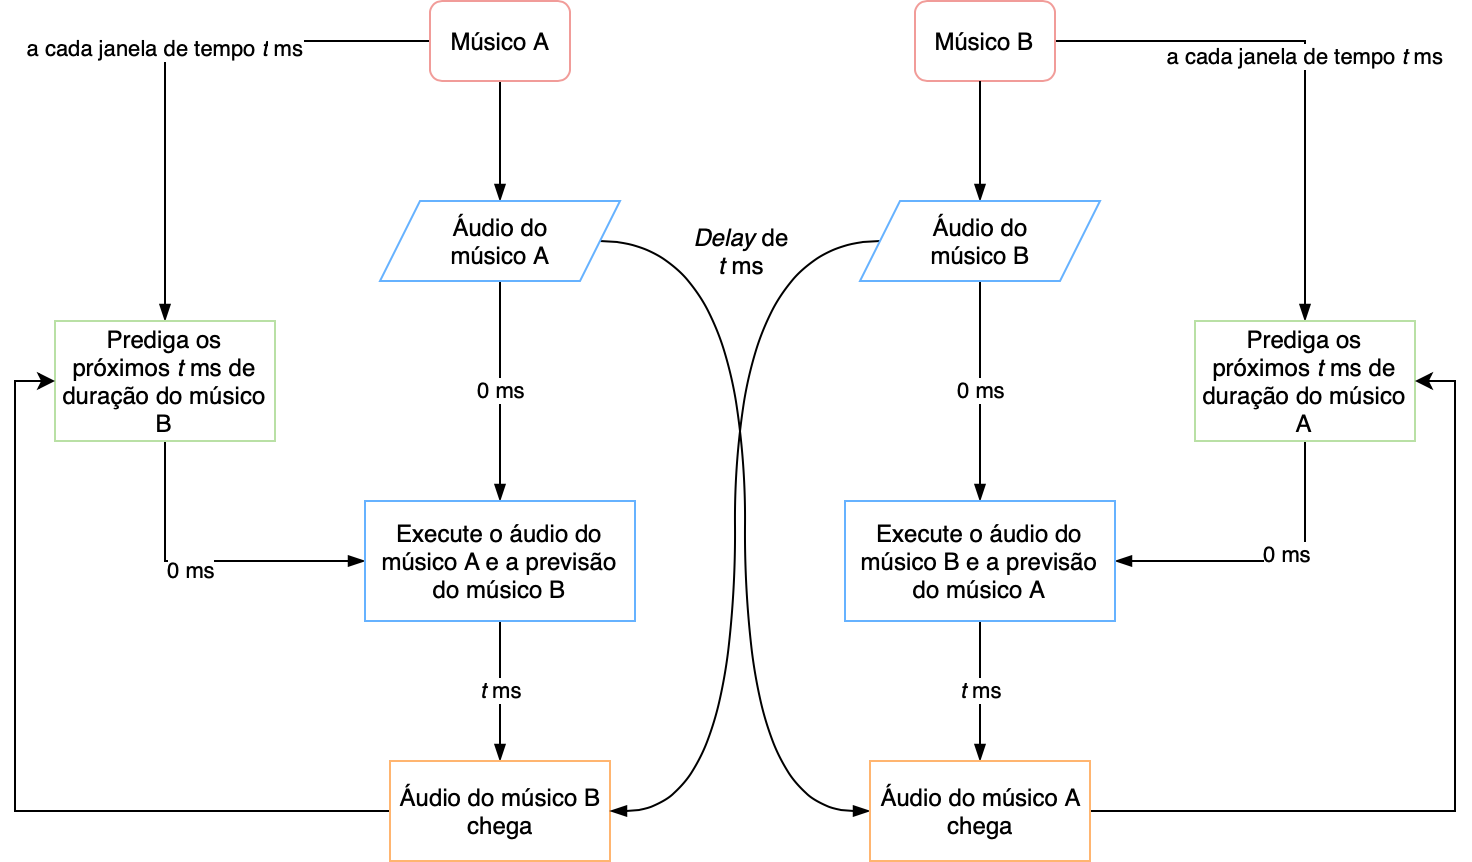
\includegraphics[width=1\textwidth]{images/rollback-music.png}
\caption{Diagrama demonstrando a adaptação do algoritmo de previsão no lado do cliente aplicado para \textit{streaming} colaborativo de música \textit{online}. Na imagem, "X" representa a duração da janela de previsão, medido em milissegundos.}
\label{fig:rollback_music_diagram}
\end{figure}

Em Bernier, a janela de tempo de cada conjunto de previsões é definida de acordo com o FPS e a velocidade de conexão entre os participantes. Na adaptação musical, além do tempo de ida e volta dos pacotes entre os participantes (\textit{ping}), propomos a utilização de outros parâmetros para a decisão dessa janela, como o BPM (batimentos da música) ou valores arbitrários. A escolha dessa janela é fundamental - durações muito longas possuem muita informação, porém, são mais difíceis de processar; e o inverso ocorre para janelas muito curtas.

Propomos, portanto, dois modelos preditivos para música, dividido em dois ciclos de pesquisa. No (CITAR CAPITULO), utilizamos a arquitetura de aprendizagem de máquina em camadas LSTM (\textit{Long short-term memory)} \cite{lstm} para gerar sequências de sinais digitais. Já em (CITAR CAPITULO), no segundo ciclo, usamos o algoritmo DTW (\textit{Dynamic Time Warping}) \cite{dtw} para identificar janelas semelhantes em uma base de dados e, a partir dessa informação, reproduzir a próxima janela de áudio, também armazenada na mesma base de dados.


% Ao observar o contexto de videogames, encontramos requisitos de latência similares. Gêneros que utilizam reações como mecânica de jogabilidade, como luta e FPS (\textit{first-person shooter}), para oferecerem aos jogadores uma experiência fluida, necessitam de latências máximas de até 100 ms \cite{pubnub}. O algoritmo mais popular e efetivo para solucionar esse problema, \textit{client-side prediction} \cite{client-side-prediction}, baseia-se em prever os próximos \textit{inputs} imediatos dos jogadores e agindo antes mesmo que os dados de seu oponente sejam transmitidos; desta forma, removendo a necessidade inicial de espera. Uma vez que os \textit{inputs} são recebidos, estes são comparados com a previsão realizada e, caso sejam incongruentes entre si, o jogo é retornado ao estado anterior do momento da previsão inicial.

% Por possuir requisitos semelhantes de baixa latência, a mesma implementação baseada em previsões tem o potencial de resolver o problema descrito anteriormente para ambientes musicais colaborativos \textit{online}. Caso seja possível prever os próximos sinais digitais produzidos pelos artistas remotos, não haveria necessidade de espera e, portanto, a latência de rede tornaria-se irrelevante.

% Evidentemente, as diferenças entre os contextos de \textit{videogames} e práticas musicais não são negligenciáveis. Ao contrário dos jogos, por apresentar uma linearidade no tempo, não é possível retornar ao último momento da música anterior à previsão imediata sem atrapalhar a performance dos artistas. Além disso, a natureza discreta dos \textit{inputs} dos \textit{videogames} e a quantidade bruta de dados produzida é ínfima em comparação à áudios digitais - estima-se que os jogadores profissionais de \textit{Super Smash Bros. Melee} mais técnicos produzem em média 6 \textit{inputs} por segundo \cite{melee_inputs_per_second}; uma transmissão de áudio com \textit{sample rate} de 44,1 khz produz, por definição, 44.100 diferentes valores no mesmo espaço de tempo \cite{jukebox_dimension}. Portanto, a aplicação do algoritmo de \textit{client-side prediction} para transmissão de música \textit{online} não é trivial, e a necessidade que o modelo preditivo seja o mais acurado possível é ainda mais importante.
\chapter{Ciclo 1: Geração de novas sequências com LSTM}
\label{chap:lstm}
\chapter{Ciclo 2: Indexação com DTW}

TODO: explicar a ideia do DTW vinda a partir dos resultados do primeiro ciclo
\chapter{Conclusões}
\label{chap:conclusion}

De acordo com nosso experimentos, o modelo preditivo gerador de novas sequências com LSTM não teve bom desempenho em nenhuma das duas métricas de sucesso estabelecidas na \secref{sec:success_metrics}. Por repetir os dados de entrada, caso utilizássemos esse modelo em uma aplicação real, estaríamos apenas atrasando o áudio transmitido e replicando o problemas que as soluções síncronas enfrentam hoje.

Além disso, devido ao alto tempo necessário para realizar a predição, tal solução mostrou-se inviável da forma que foi implementada. Para atingir tempos menores, seria necessário mais poder computacional, tornando essa solução inacessível para a população em geral.

Portanto, de acordo com nossos experimentos, o modelo gerador com LSTM não se mostrou promissor para ser utilizado em uma adaptação do \textit{client-side prediction} para ambientes musicais. Porém, melhorias podem ser estudadas que viabilizem seu uso, exploradas na \secref{sec:later_work}.

Entretanto, no segundo ciclo, o modelo indexador e identificador mostrou-se bastante promissor em nossos experimentos. Apesar de possuir uma base da dados pequena, a taxa de acerto das previsões foi consideravelmente alta, de forma a trazer a sensação de fluidez nos momentos de acerto na previsão. Se relacionarmos com o \textit{client-side prediction}, que corrige os \textit{inputs} dos jogadores sempre que há um erro, os erros nas previsões realizadas podem ser aceitáveis.

Ademais, o tempo necessário para apontar as predições foi bastante baixo, deixando espaço suficiente para que máquinas menos potentes do que a utilizada nos experimentos possam usufruir dessa abordagem.

Porém, não podemos afirmar com certeza suficiente que o modelo indexador pode ser utilizado em aplicações reais. A base de dados utilizada foi propositalmente reduzida para testar a validade do modelo, possibilitando altas taxas de acertos na identificação e alta eficiência. Além disso, as janelas de áudio escolhidas são consideravelmente altas, o que impede seu uso em improvisações musicais.

Entretanto, o modelo indexador com DTW mostrou-se bastante promissor para uso na adaptação do \textit{client-side prediction} para ambientes musicais, principalmente para músicos de base, que não tendem a improvisar em suas performances.



%%
%% Parte pós-textual
%%
\backmatter

% Apêndices
% Comente se não houver apêndices
\appendix

% É aconselhável criar cada apêndice em um arquivo à parte, digamos
% "apendice1.tex", "apendice.tex", ... "apendiceM.tex" e depois
% incluí-los com:
% \include{apendice1}
% \include{apendice2}
% ...
% \include{apendiceM}


% Bibliografia
% É aconselhável utilizar o BibTeX a partir de um arquivo, digamos "biblio.bib".
% Para ajuda na criação do arquivo .bib e utilização do BibTeX, recorra ao
% BibTeXpress em www.cin.ufpe.br/~paguso/bibtexpress
\nocite{*}
\bibliographystyle{ieeetr}
\bibliography{references}

% Cólofon
% Inclui uma pequena nota com referência à UFPEThesis
% Comente para omitir
% \colophon

%% Fim do documento
\end{document}
